

\lesson{2}{15.09.2023}{Бинарные отношения}

\section{Бинарные отношения}



\begin{definition}
    Бинарноным отношением между множествами X и Y называют подмножество $X \times Y$

\end{definition}

\begin{notation}
    Пусть задано $w \subset X \times Y$. Тогда, условие $(x, y) \in w$ записывается как $X w Y$
\end{notation}

\begin{notation}
    Если X = Y, то говорят, что w - отношение на X.
\end{notation}

\begin{proof}
    \begin{figure}[H]
        \centering
        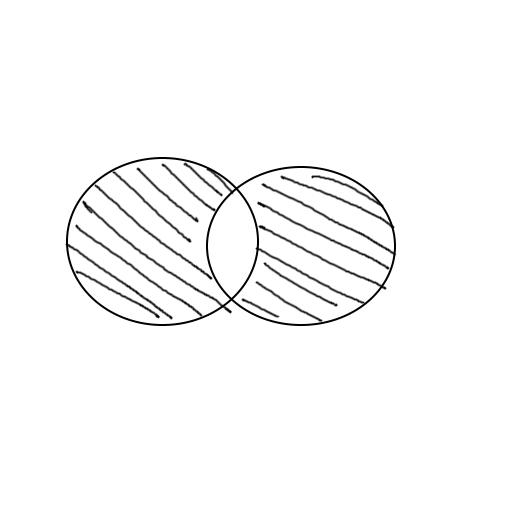
\includegraphics[width=\linewidth]{1.png}
        
        
        \label{fig:1}
    \end{figure}

    Пусть $g_1, g_2$ - отображения к R.

    $q_1 \neq q_2$

    $\exists g : g, (g) \neq g = (g)$

    $x_i = y_1(y), x_2 := g_2(y)$

    $f(x_1) = f(g_1(y)) = g = f(g_2(y)) = f(x_2)$

    $f(x_1) = f(x_2)$

    $x_1 \neq x_2$
\end{proof}

\begin{eg}
    \begin{enumerate}
        \item $f(x) = 2x$
        
        $ x w y$, если $g = f(x)$

        \begin{figure}[H]
            \centering
            
\includegraphics[width=\linewidth]{2.png}
            
            
            \label{fig:2}
        \end{figure}

        \item $x w y$, если $x^2 = y$
        
        \begin{figure}[H]
            \centering
            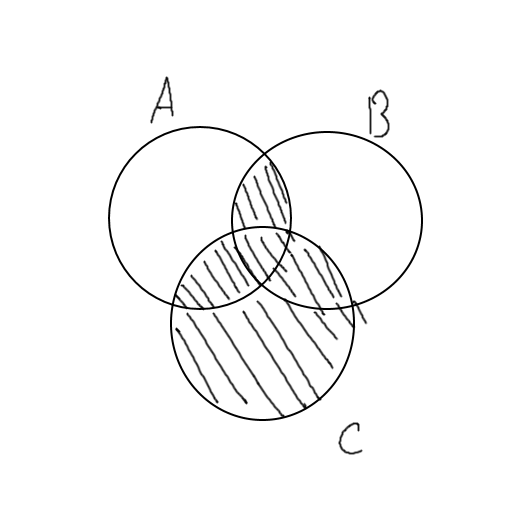
\includegraphics[width=\linewidth]{3.png}
            
            
            \label{fig:3}
        \end{figure}
    \end{enumerate}
\end{eg}

\begin{definition}
    Бинарное отношения w на X называется

    \begin{enumerate}
        \item Рефлексивным, если $x w y$ и $y w z$
        \item Симметричным, если из того что $x w y$ и $y w z$ следует, что $x w f$
    \end{enumerate}
\end{definition}

\begin{eg}
    \begin{enumerate}
        \item $=, \leq$ - рефлексивное
        
        <, паралленльно на множестве прямых - не рефлексивно
        \item $=, ||$ - симметрично
        
        $leq, <$ - не симметрично
        \item $=, <, \vdots$ - транзитивно
        
        $\perp$ - на множестве прямх - не транзитивно 
    \end{enumerate}
\end{eg}

\begin{definition}
    Бинарное отношение на множестве X называется отношением эквивалентности, если оно рефлексивно, симметрично и транзитивно.

\end{definition}

\begin{notation}
    
    Обычно обозначается $\sim$.

\end{notation}

\begin{eg}
    
    \begin{enumerate}
        \item = на $\R$
        \item Множество $\Z$ $a \sim b$, если $a - b \vdots 5$
        \begin{notation}
            $\overline {\overline {\overline {5}}}$
        \end{notation}
        \item Множество проямых на плоскости $l_1 \sim l_2$, если $l_2 || l_2'$, если $L_1 = l_2$
        \item Пусть множество - это множество направленных отрезков $\overline{AB}  \sim \overline{CD}$, если $|\overline{AB}| = |\overline{CD}|$, $AB || CD$.
        \item $f(x),g(x)$ - функции $f \sim g$, если $\lim_{x\to\infty}\frac{f(x)}{f(y)} = 1$
    \end{enumerate}

\end{eg}

\begin{definition}
    Пусть на X задано отношение эквивалентности. Классом эквивалентности x называется множество элементов $\{y \in X | y \sim X\}$.
\end{definition}

\begin{notation}
    $\overline{x}$, $[x]$, $((x)$

    \begin{note}
        Черта над x должна быть немного загнута вниз слева. Также первый вариант обозначения является основным.
    \end{note}
\end{notation}

\begin{eg}
$R, x \sim y, если x - y \in \Z$

$x = 0, 1$

0,1; 1,1;$-0.9 \in \overline x$

$\overline x = \{ y | \{y\} = \{x\}\}$
\end{eg}

\begin{eg}
    $1,1 \in \overline{0, 1}$

    $0,1 \in \overline{1, 1}$

    \{y\} = 0, 1
\end{eg}

5 классов эквивалентности:

5k

5k + 1

5k + 2

5k + 3

5k + 4

\begin{theorem} (Разбиение на классы жкивалентности)
На множестве X задано отношение эквивалентности ~. Тогда, множество X разбивается на классы эквивалентности, т.е. X является обьединением не пересекающихся подмножеств, каждое из которых является классом эквивалентности некоторого элемента.
\end{theorem}

\begin{eg}

    
\begin{enumerate}

    \item $\overline {\overline {\overline {5}}}$
    
    $a \sim b$, если $a - b \vdots 5$
    \item = в каждом классе 1 элемент
    
    \item Направленные отрезки $overline{AB} \sim \overline{CD}$, если $|\overline{AB}| = |\overline{CD}|$, $AB \uparrow\uparrow CD$
    

    Класс эквивалентности - вектор.
    \item R $a \sim b$, если $\alpha - \beta = 2 \pi \kappa$
    \begin{figure}[H]
        \centering
        
\includegraphics[width=\linewidth]{4.png}
        
        
        \label{fig:4}
    \end{figure}
\end{enumerate}
\end{eg}

\begin{proof}
    \begin{enumerate}
        \item Докажем, что любой элемент X принадлежит некоторому классу эквивалентности.

        $X \in \overline X$, т.к. $\sim$ ???, X ~ x

        \item Докажем, что классы не пересекаются
        
        \begin{figure}[H]
            \centering
            
\includegraphics[width=\linewidth]{5.png}
            
            
            \label{fig:5}
        \end{figure}

        т.е. докажем, что если $\exists z \in \overline x \cap \overline y$, то $\overline x = \overline y$

        \begin{figure}[H]
            \centering
            
\includegraphics[width=\linewidth]{6.png}
            
            
            \label{fig:6}
        \end{figure}

        $z \in x$ => $z \sim x$ => (симм) $x \sim z$

        $z \in \overline y$ => z ~ Y

        x ~ z, z ~ y => (тр) x ~ y => $x \in y$ => $x \in \overline y$

        аналогично $y \in \overline x$
    \end{enumerate}
    
    \begin{figure}[H]
        \centering
        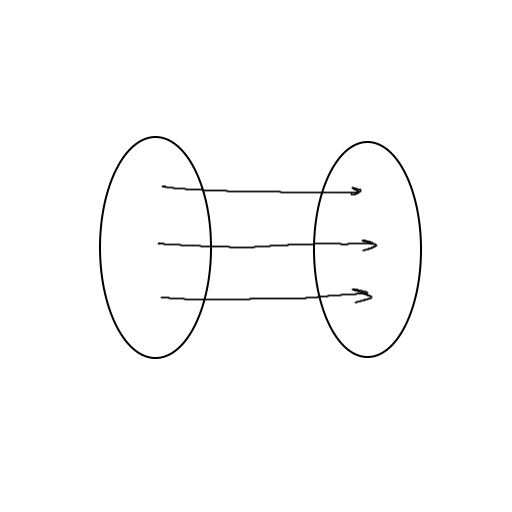
\includegraphics[width=\linewidth]{7.png}
        
        
        \label{fig:7}
    \end{figure}

    $x = \overline y$

    Докажем, что $ \overline x \subset y$

    Пусть $\exists f \in \overline x => f \sim x$

    $f \sim x, x = y => f \sim y$

    Аналогично $\overline y \subset \overline x$

    $\overline x = \overline y$
\end{proof}

\section{Множество с алгебраическими операциями}

\begin{definition}
    X - множество бинарныой алгебраической операции на X Назвается отображением $X \times X \to X$
    
    
\end{definition}

\begin{notation}
    \begin{enumerate}
        \item Буква, например $f : X \times X \to X$
        пишут $f(x, y)$ или $x f y$

        \item Спец. символ: +, $\cdot$, 0, *
        Пишут x + y, x * y

        часто вместо $x \cdot y$, x * y пишут xy
    \end{enumerate}

    
\end{notation}

\begin{eg}
\begin{enumerate}
    \item $X = \Z$
    
    Определить +, $\cdot$, -

    \item X - множество отображений $\Z \to \Z$,
    
    операция - композиция.

    \item X - множество векторов
    
\end{enumerate}
\end{eg}

\begin{notation}
    Множество X с операцией V обозначается (V, *)
\end{notation}

\begin{definition}
    Бинарная операция * на X Назвается

    \begin{enumerate}
        \item Ассоциативной, если $(x * y * z) = x * (y * z) \forall x, y, z$
        
        \item Коммутативной, если $x * y = y * x \forall x, y$
    \end{enumerate}
\end{definition}

\begin{eg}

\begin{enumerate}
    \item +, $\cdot$ - коммутативные, ассоциативные 
    
    X : y на $\R \setminus \{0\}$ не ассоциативно, не коммутативно

    x - y на $\R$

    x - векторное произведение

    \item ассоциативны, не коммутативны
    o - композиция для отображения $\Z \to \Z$

\end{enumerate}

\end{eg}

\begin{notation}
    Пусть * - ассоциативно

    Тогда пишут a * b * c, a * b * c * d

    Используют обозначение степени, например $a^4$ = a * a * a * a

    Если операция обозначается +, пишут

    $4a = a + a + a + a$


\end{notation}

\begin{eg}
    \begin{enumerate}
        \item (Z, $\cdot$) e = 1
        \item (Z, +) e = 0
        \item (2Z, $\cdot$) нет ? элемента, множества четных чисел
    \end{enumerate}
\end{eg}

\begin{remark}
    Если операция обозначается +, то неитральный элемент обозначается 0.
\end{remark}

\begin{property} (единственности единичного элемента)

    На x Задана операция *. Тогда существует не более одного единичного элемента.
\end{property}

\begin{proof}
    Пусть $e_1, e_2$ - единичные, т.е.

    $\forall_x$
    $e_1 + x = x, x + e_1 = x$
    $e_2 * x = x, x * e_2 = x$

    $e_2 = $(ед. эл.)$ e_1 * e_2 = $(ед.эл.)$ e_1 => e_1 = e_2$


\end{proof}

\begin{definition}
    Полугруппой называется множество с заданной на нем бинарной ассоциативной операцией.
\end{definition}

\begin{definition}
    Моноидом называется полугруппа, в которой есть неитральный элемент
\end{definition}

\begin{eg}
    \begin{enumerate}
        \item ($\Z$, +) - моноид
        \item (Z, $\cdot$) - моноид
        \item ($2\Z$, $\cdot$) - полугруппа, не моноид
        \item ($\Z$, -) - вектор $\subset x$ - не полугруппа
    \end{enumerate}
\end{eg}

\section{Группы}

\begin{definition}
    Множество G с бинарной операцией * называется группой, если выполнены следующие условия.

    \begin{enumerate}
        \item Операция * ассоциативна, т.е. (a * e) * c = a * (b * c) $\forall a, b, c$
        \item $\exists$ единица $e: a * e = e * a = a \forall a$
        \item $\forall a \exists$ Обратный элемент a' $\in G$ такой, что $a * a^-1 = a^-1 * a = e$
    \end{enumerate}
\end{definition}

\begin{notation}
    Если операция обозначается -1, то единичные жлементы обозначаются o, а обратный элемент a обозначается -a.
\end{notation}

\begin{definition}
    Пусть (G, *) - группа, если * коммутативна, то группа G называется коммутативной или абелевой.
\end{definition}
